\documentclass[11pt]{article}

\usepackage{setspace}
\usepackage[margin=1in]{geometry}
\usepackage{graphicx}
\usepackage{amsmath}
\usepackage{mathtools}
\usepackage{natbib} %for citet and citep
\usepackage{syntonly}
\usepackage{esdiff} %for writing partial derivatives
\usepackage{url} %for inserting urls
\usepackage{placeins}
\usepackage{textcomp} % for tildas
% \syntaxonly for quickly checking document
%set document settings

 \doublespacing % from package setspacs

% table font size
\let\oldtabular\tabular
\renewcommand{\tabular}{\scriptsize\oldtabular}

\title{Wind farm investment under spatial uncertainty: A Bayesian model with an option of waiting}

\author{Jostein Lillest\o l \& Johannes Mauritzen\\
 		Department of Business and Management Science\\
   NHH Norwegian School of Economics\\
   Bergen, Norway\\
%   johannes.mauritzen@nhh.no\\
%   \url{jmaurit.github.io}\\
		}
\date{\today}


\begin{document}

\begin{spacing}{1} %sets spacing to single for title page

\maketitle

\begin{abstract}
 ...
\end{abstract}

\thanks{*We would like to thank Endre Bj\o rndal, Jonas Andersson, and Gunnar Eskeland for helpful comments and suggestions. Data has been generously provided by Kjeller Vindteknikk. Financial support has been received from the Research Council of Norway through the projects INTREPID and CenSES.}
%JEL Codes: Q4, L71
\end{spacing}

\section{Introduction}

Unlike traditional energy generation technologies, the efficiency and profitability of wind turbines and wind farms are highly dependent on their location. Even modest differences in long-term average wind speeds can have major consequences on the profitability of wind farms over time. However, the inherent appropriateness of a given location is subject to a high degree of uncertainty as wind speeds can vary substantially even within areas where overall wind resources are good. More so, average wind speeds show a high degree of variance from month-to-month and even year-to-year.

The high degree of spatial and temporal variation of wind speeds leads to large uncertainty when making wind farm investment decisions. In this article we propose a simple sequential Bayesian decision model that takes into account spatial uncertainty and allows for the option of waiting to collect more information on wind speeds.

We first introduce a simple two period toy model with linear loss function. This simple model can be solved analytically, generating some stylized results that provide intuition and a frameworks for interpreting more complicated models. 

We then introduce a case study with data from a proposed wind farm in Northern Norway. We introduce realistic wind turbine power output function and investment loss functions that reflect the real-life non-linear relationship between wind-speeds and power generation. 

We use the Bayesian posterior sampling and modeling language Stan \citep{stan_development_team_stan} to simulate sampling from the posterior. This approach allows the model to be easily extended to take into account, for example, price and regulatory uncertainty - though for the sake of brevity and clarity, we do not pursue these extensions here.


\section{Analytic Frameworks}


\section{Case Study: The Andmyran Wind Farm in Northern Norway}

We consider the case of the proposed Andmyran wind farm, located on an island in northern Norway. To establish the basis for the prior beliefs about the wind resources of the given location, we gather publicly available information on average wind speeds from three nearby weather stations: Andenes, Harstad and Sortland. This is obtained from the website of the Norwegian Meteorological Society's public weather page, \url{yr.no}. 

Figure \ref{avg_wind_speed_data} shows a chart of the average monthly wind speeds for the three sites. We can note the significant variation in average wind speed between the sites, even though they are all within 50 kilometers of one another. 

\begin{figure}
	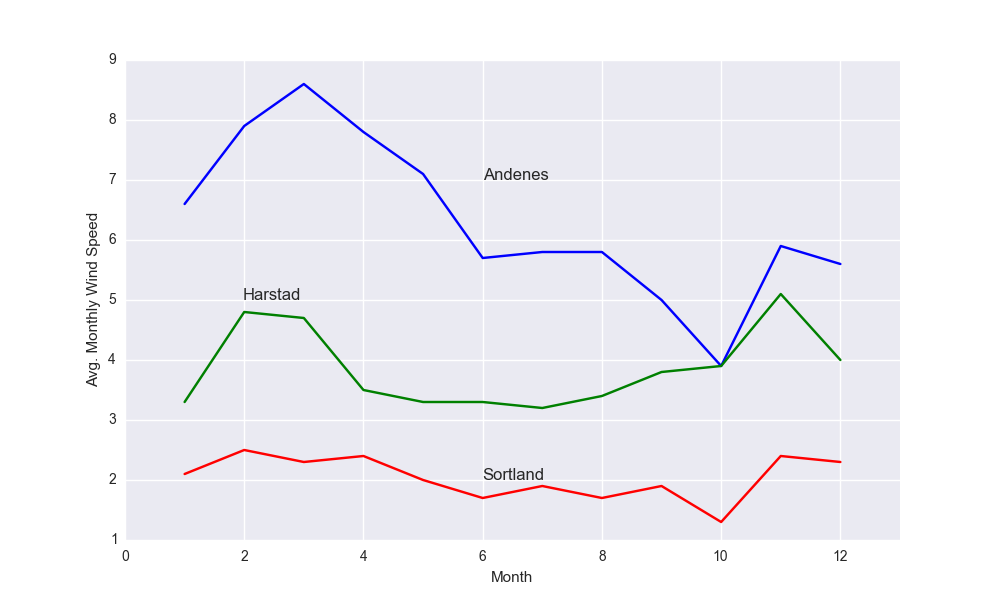
\includegraphics[width=1\textwidth]{figures/avg_wind_speed_data.png}
	\caption{Average monthly wind speeds from the three closest weather stations to the proposed Andymren site.}
	\label{avg_wind_speed_data}
\end{figure}

Wind speeds measured at shorter intervals are known to roughly follow a weibull distribution \footnote{A weibull distribution is defined as having a probability distribution function of $f(x, \lambda, k) = \frac{k}{\lambda} \frac{x}{\lambda}^{k-1} e^{-\frac{x}{\lambda}^k}$}. Thus we use the formula for the mean of a weibull distribution, as shown in equation \ref{mean_weibull}. Here $Gamma$ represents the Gamma function.

\begin{equation}
\mu_{weibull} = k*Gamma(1+\frac{1}{\lambda})^2
\label{mean_weibull}
\end{equation}

A simple least-squares optimisation routine is run in order to choose point estimates for the $k$ and $\lambda$ values of a weibull distribution that best fit the data on monthly average wind speeds. From this optimisation, estimates of the shape parameter $k_hat = .6$ and the scale parameter $lambda_hat = 3.2$ are found.  This corresponds to a weibull distribution with the pdf as shown in figure \ref{avg_wind_speed_data}. A histogram of one year of hourly measurements (8760) are plotted along the probability distribution. 

\begin{figure}
	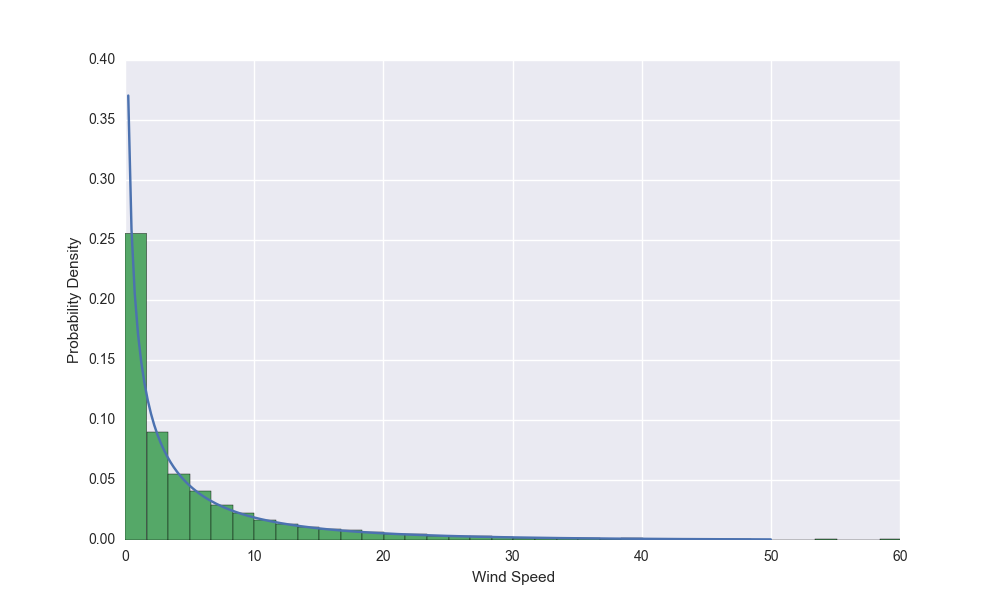
\includegraphics[width=1\textwidth]{figures/prior_distribution.png}
	\caption{Weibull probability distribution of the prior predictive distribution of wind speeds for Andmyran. The histogram represents 8640 random draws from the distribution, consisting of one year of hourly measurements.}
	\label{avg_wind_speed_data}
\end{figure}

To transform the simulated wind speed data from the weibull distribution to power output data, I use the power curve of a common commercial wind turbine: the Vestas V90 turbine. The power curve can be seen in the top panel of figure \ref{power_output}. At wind speeds up to 4 meters per second (m/s), no power is produced. Between speeds of 4 and 15 m/s, power output rapidly increases with respect to wind speed. The rated power output is reached at wind speeds of between 15 and 25 m/s, after which power is cut-out in order to protect the turbine. 

\begin{figure}
	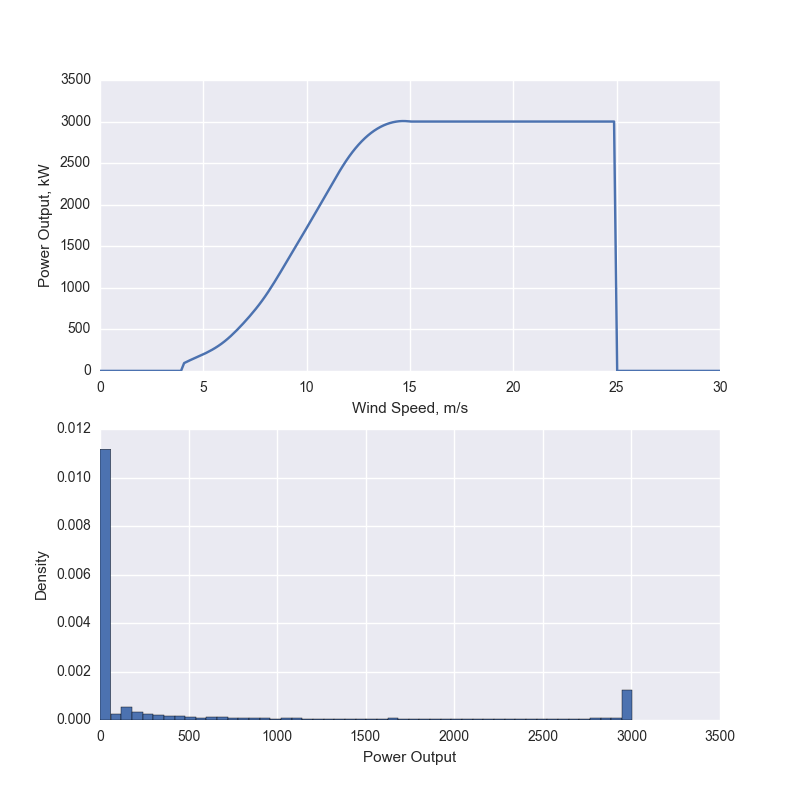
\includegraphics[width=1\textwidth]{figures/power_output.png}
	\caption{Weibull probability distribution of the prior predictive distribution of wind speeds for Andmyran. The histogram represents 8640 random draws from the distribution, consisting of one year of hourly measurements.}
	\label{power_output}
\end{figure}

The lower panel of figure \ref{power_output} shows the histogram of power outputs. We can notice the high number of hours with zero production.

The loss functions are defined as in equation \ref{loss_functions}:

\begin{align}
L_{invest} = I - (p_{kwh} - c_{kwh})*kwh\\
L_{pass} = d((p_{kwh} - c_{kwh})*kwh-I)\\
L_{wait-invest} = M + I - (p_{kwh} - c_{kwh})*kwh\\
L_{wait-pass} = M + I - d(p_{kwh} - c_{kwh})*kwh
\label{loss_functions}
\end{align}

These functions describe the losses associated with investing or passing in the first period as well as waiting and then deciding. $I$ represents the lump-sum investment cost, $p_KWH$ is the price per kilowatt-hour (kWh) for the electricity produced. $c_kwh$ represents any running costs. $d$ represents a discount rate on the opportunity cost of not investing - the intuition here is that the capital could be put in place in some other investment that gains a return. $M$ represents the cost associated with waiting and gathering data. This could include the cost of installing and monitoring a wind-measuring station.

Given the loss functions for the different choices with parameters: $I=100,000$, $c_{oper}=0.005$, $p_{kwh}$, $d=.90$, $M=0$ we then draw 500 sample years of hourly wind data. At the first stage the investor can either choose to invest, to pass, or to wait and gather more information. The distribution of the losses for each sampled year for these three choices are shown in figure \ref{losses}.

\begin{figure}
	\centering
	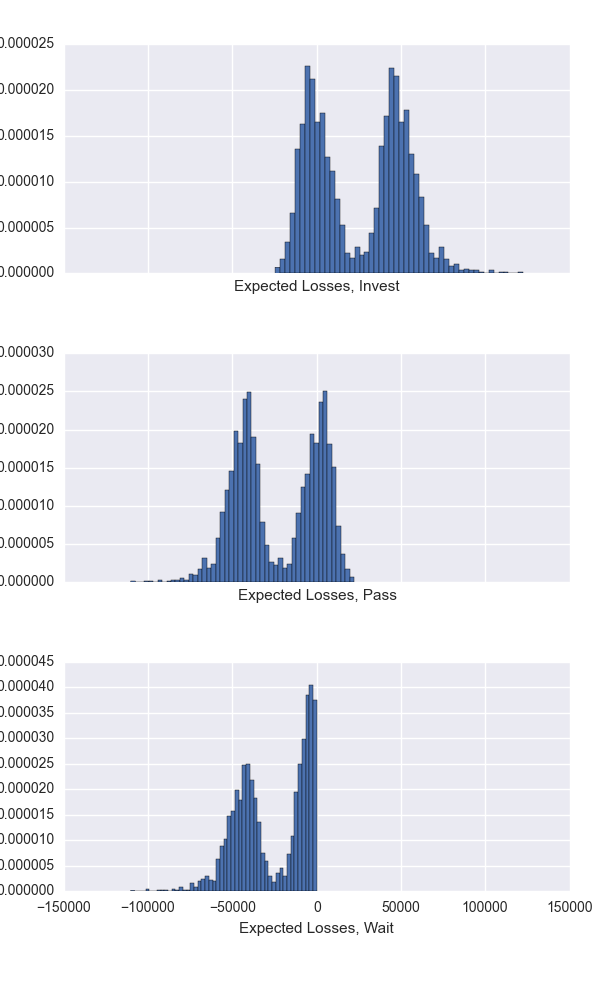
\includegraphics[width=.6\textwidth]{figures/losses.png}
	\caption{Distribution of losses for the decisions to invest, pass or wait.}
	\label{losses}
\end{figure}

With the chosen parameters there is a high degree of prior uncertainty about whether a project will be profitable or not. Thus there is a high degree of value in waiting. The strong assumption in calculating the expected loss of waiting is that the investor will know with certainty whether investing is profitable or not after having gathered more information. This is why the expected loss of waiting in this simulation is always less than zero.

Taking the expected value of each distribution from this particular case, we get the values shown in table \ref{table:expected_losses}. Clearly, the value of waiting in this example are quite high. One way of interpreting the result would be to say that it would be worthwhile to wait and gather more information if the cost of gathering the information, $M$ were less than 1539 (1609-70.4.) Otherwise, you would pass on making the investment. 

\begin{table}
\begin{center}
\begin{tabular}{l c}
$E(loss_{invest})$ & 78.3 \\
$E(loss_{pass})$ & -70.4 \\
$E(loss_{wait})$ & -1609.4 \\

\end{tabular}
\caption{Expected losses from decision to invest, pass or wait at first stage}
\label{table:expected_losses}
\end{center}
\end{table}

Having decided to wait and gather more information, the next step is then to update the prior distribution with the gathered data and obtain a posterior distribution with which to make a new investment decision.

The simple model can be expressed as in equation \ref{bayes_model}. The first term expresses the likelihood as a weibull function with shape parameter $\alpha$ and scale parameter $\sigma$. In turn these parameters are given informative prior distributions with means $\hat{\alpha}$ and $\hat{\sigma}$ that are estimated from the publicly available data on average wind speeds in the area, as detailed earlier.   

\begin{align}
p(wind-data|\theta) &\sim weibull(\alpha, \sigma)\\
alpha &\sim normal(\hat{\alpha}, 1)\\
sigma &\sim normal(\hat{\sigma}, 1)
\label{bayes_model}
\end{align}

To sample from the posterior distribution $p(alpha, sigma|wind-data)$ we use the bayesian programming language and Markov Chain Monte Carlo (MCMC) sampler Stan. Stan utilizes Hamiltonian Monte Carlo to efficiently simulate sampling from the posterior. 

Other popular simulation tools are widely available like BUGS and JAGS, but we chose to use Stan because of the flexibility of its modeling language and the efficiency of its sampling routine. While the case outlined hear is quite simple, the model can be easily extended with Stan to include other sources of uncertainty relevant to the real-life investment decision.

The wind data is taken from actual wind measurement data at the appropriate height at the sight of the proposed Andmyran wind farm. We use 1 year of hourly measurements - or 8780 data points in the updating of the posterior distribution. 

Figure \ref{posteriors} shows a histogram of draws from the posterior distributions of the shape parameter $\alpha$ in the top panel and the scale paramter $\sigma$.

\begin{figure}
	\centering
	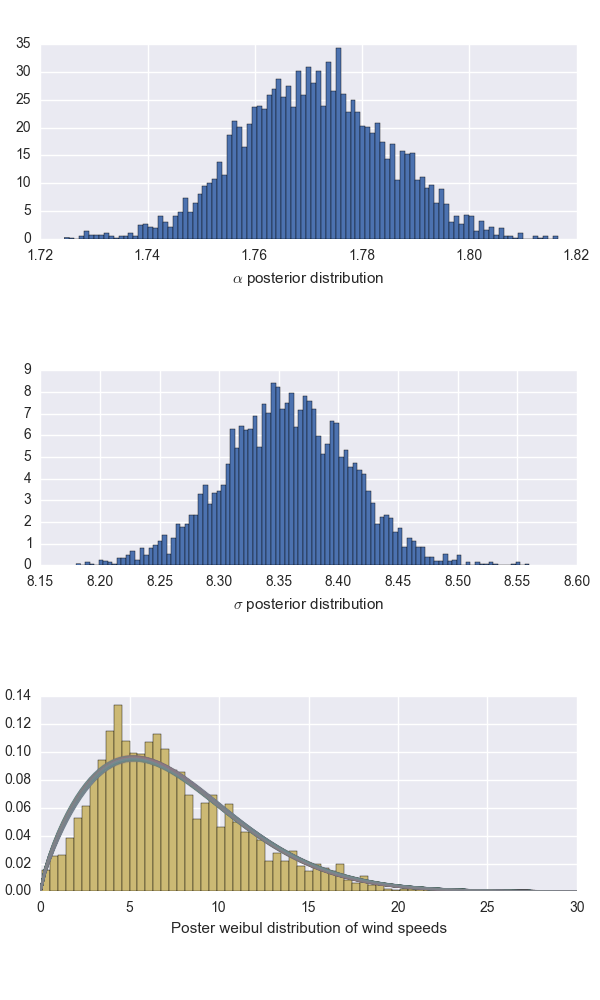
\includegraphics[width=.6\textwidth]{figures/posteriors.png}
	\caption{Posterior distributions of the $\alpha$ (top panel) and $\sigma$ (middle panel) parameter of the weibull distribution. The bottom panel shows the weibul distribution with draws from the $\alpha$ and $\sigma$ posterior distributions. The histogram of the actual data is overlaid.}
	\label{posteriors}
\end{figure}

To simulate wind speeds from the posterior distribution, we first draw values of $\alpha_{draw}$ and $\sigma_{draw}$ from their posterior distribution. We then draw 8760 simulated wind speed observations from a $weibull(\alpha_{draw}, \sigma_{draw})$ distribution, representing a year of hourly observations. These values are converted to power output with the power curve function detailed earlier. The power output is then summed and returned. We then repeat this to generate a measure of uncertainty over the yearly wind conditions.

From this sample of of yearly wind conditions, we calculate a sample of expected losses for the second stage decisions of whether to invest or pass. The results are shown in the form of histograms in figure \ref{post_losses}. The updated posterior beliefs indicates that the investment will be profitable with high certainty. 

\begin{figure}
	\centering
	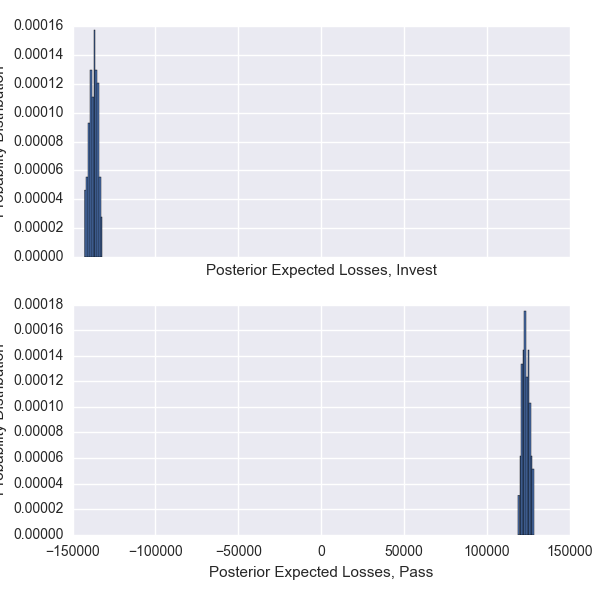
\includegraphics[width=.8\textwidth]{figures/post_losses.png}
	\caption{Posterior distribution of expected losses. Investing is now expected to be profitable with high certainty.}
	\label{post_losses}
\end{figure}


\section{Conclusion}
This article has three main contributions. First, it recognizes that wind power investments decisions, and potentially other renewable energy decisions, are subject to a large degree of spatial uncertainty. Even with the case study of a proposed site in a region which has some of the best average wind resources in the world, a high degree of uncertainty exists about the viability of any given project. While this point is more or less common sense in the industry, it has not been widely acknowledged in the literature, and it is not, to our knowledge, included in explicit academic models of wind power investment. 

The second contribution is to model the sequential nature of a wind power investment by way of a Bayesian decision model where the spatial uncertainty can be modeled explicitly and where the option of waiting and gathering more data in order to update prior beliefs can be modeled naturally. 

Finally, our implementation of the model using the open and flexible Bayesian modeling language and MCMC sampler Stan allows for straight-forward extensions that allows for me realism in the model. We hope and expect that the model could be easily extended by both other academics and we hope investors looking for a way to formalize their decision making processes.  We have posted all our code at \url{jmaurit.github.io#wind_invest_model}.
 
\begin{spacing}{1}
\bibliographystyle{plainnat}
\bibliography{wind_investment}
\end{spacing}

\end{document}


